% utf-8 ru, unix eolns
\documentclass[12pt,a4paper,oneside]{extarticle}
    \righthyphenmin=2 %минимально переносится 2 символа %%%
    \sloppy

% Рукопись оформлена в соответствии с правилами оформления 
% электронной версии авторского оригинала, 
% принятыми в Издательстве МГТУ им. Н.Э. Баумана.

\usepackage{geometry} % А4, примерно 28-31 строк(а) на странице 
    \geometry{paper=a4paper}
    \geometry{includehead=false} % Нет верх. колонтитула
    \geometry{includefoot=true}  % Есть номер страницы
    \geometry{bindingoffset=0mm} % Переплет    : 0  мм
    \geometry{top=20mm}          % Поле верхнее: 20 мм
    \geometry{bottom=25mm}       % Поле нижнее : 25 мм 
    \geometry{left=25mm}         % Поле левое  : 25 мм
    \geometry{right=25mm}        % Поле правое : 25 мм
    \geometry{headsep=10mm}  % От края до верх. колонтитула: 10 мм
    \geometry{footskip=20mm} % От края до нижн. колонтитула: 20 мм 

\usepackage{cmap}
\usepackage[T2A]{fontenc} 
\usepackage[utf8x]{inputenc}
\usepackage[english,russian]{babel}
\usepackage{misccorr}

\usepackage{amsmath}
\usepackage{amsfonts}
\usepackage{amssymb}

%\usepackage{cm-super} %человеческий рендер русских шрифтов

\setlength{\parindent}{1.25cm}  % Абзацный отступ: 1,25 см
\usepackage{indentfirst}        % 1-й абзац имеет отступ

\usepackage{setspace}   

\onehalfspacing % Полуторный интервал между строками

\makeatletter
\renewcommand{\@oddfoot }{\hfil\thepage\hfil} % Номер стр.
\renewcommand{\@evenfoot}{\hfil\thepage\hfil} % Номер стр.
\renewcommand{\@oddhead }{} % Нет верх. колонтитула
\renewcommand{\@evenhead}{} % Нет верх. колонтитула
\makeatother

\usepackage{fancyvrb}

\usepackage[nounderscore]{syntax} %для поддержки рбнф
%\setlength{\grammarindent}{12em} %устанавливает нужный отступ перед ::=
\setlength{\grammarparsep}{6pt plus 1pt minus 1pt}  %сокращает расстояние между правилами

\usepackage[pdftex]{graphicx}  % поддержка картинок для пдф
\graphicspath{ {./pictures/} }
\usepackage{rotating}
%\DeclareGraphicsExtensions{.jpg,.png}

\renewcommand{\labelenumi}{\theenumi.} %меняет вид нумерованного списка

\usepackage{perpage} %нумерация сносок 
\MakePerPage{footnote}

\usepackage[all]{xy} %поддержка графов

\usepackage{listings} %листинги
\renewcommand{\lstlistingname}{Листинг}

\usepackage{url}


\usepackage{tikz} %для рисования графиков
\usepackage{pgfplots}


\usepackage{ccaption}%изменяет подпись к рисунку
\makeatletter 
\renewcommand{\fnum@figure}[1]{Рисунок~\thefigure~---~\sffamily}
\makeatother



\begin{document}
\pgfplotsset{compat=1.8}

\thispagestyle{empty}
\newpage
{
\centering


\textbf{
МОСКОВСКИЙ ГОСУДАРСТВЕННЫЙ ТЕХНИЧЕСКИЙ УНИВЕРСИТЕТ ИМЕНИ Н. Э. БАУМАНА \\
Факультет информатики и систем управления \\
Кафедра теоретической информатики и компьютерных технологий}
\bigskip
\bigskip
\bigskip
\bigskip
\bigskip
\bigskip
\bigskip

\vfill


Курсовой проект \\
по курсу <<Конструирование компиляторов>>

\bigskip

{\large <<Препроцессор синаксического сахара для языка Scheme>>}
\bigskip

\vfill



\hfill\parbox{4cm} {
Выполнил:\\
студент ИУ9-101 \hfill \\
Выборнов А. И.\hfill \medskip\\
Руководитель:\\
Дубанов А. В.\hfill
}


\vspace{\fill}

Москва \number\year
\clearpage
}


\tableofcontents

\clearpage

\begin{itemize}
    \item уточнить название работы
    \item что делать с тестированием
    \item упоминание lactose
    \item объекты и методы, мб туда внести что-то из реализации?
    \item куда вставить инфу про замыкания?
\end{itemize}

\clearpage

\section*{Введение}
\addcontentsline{toc}{section}{Введение}
    Lisp~---~это семейство динамических функциональных языков программирования.
    Первая версия языка Lisp была создана в 1958 году в ходе работ по созданию искусственного интеллекта.
    К настоящему времени сфера применения Lisp значительно увеличилась, а Lisp представляет собой целое семейство языков: Сommon Lisp, Scheme, Racket и другие. 

    В рамках работы рассматривается язык Scheme.
    Этот язык был разработан специально для учебных целей, благодаря чему включает в себя очень ограниченный, но весьма гибкий набор примитивов.
    Scheme удобен для написания скриптов и расширений~(имеется специально для этого предназначенная реализация~---~GNU Guile).

    Форматирование кода на Scheme, отслеживание парных открывающих и закрывающих скобок и некоторые другие синтаксические особенности требуют применения не слишком распространенных и привычных приложений таких как специализированная среда разработки, к примеру~---~Racket или текстовый реадактор со специальными расширениями, наиболее часто используется Emacs. 

    К числу недостатков можно также отнести: обилие скобок, затрудняющее чтение программы, отсутствие возможности записи выражений в привычном инфиксном формате.
    
    Целью данной работы является разработка и реализация функционального динамического языка на основе Scheme, который имеет более дружелюбный синтаксис.
\clearpage

\section{Теоретическая часть}
    \subsection{Scheme}
        \textcolor{red}{Поподробнее про схему.}

        схема - это ...

        racket - это ...

        такие-то основные фишки

        такие-то основные недостатки

        В данной работе порождается язык Scheme, удолетворяющая стандарту r5rs~\cite{r5rs}.
    \subsection{Входной язык}
        \textcolor{red}{вступленние}

        Программа на исходном языке представляет собой множество определений функций.

        Переменные также рассматриваются как функции.

        Входной точкой программы является функция main.

        \subsubsection{Токены}
            Токены языка аналогичны токенам языка программирования Scheme.
            Представлены следующие виды токенов: строка, идентификатор, число, логический тип и символ (литеральная константа). Примеры правильных токенов: 

            \begin{itemize}
                \item символ закрывающей скобки~---~\lstinline$#\)$
                \item строка~---~\lstinline$"\"r5rs\" standart\n"$
                \item идентификатор~---~\lstinline$_ident$
                \item логическая истина~---~\lstinline$#t$
                \item десятичное число~---~\lstinline$123$
                \item шестнадцатеричное число~---~\lstinline$#xDEADBEAF$
            \end{itemize}

            В рамках грамматики под нетерминалом $\langle token\rangle$ подразумевают строку, число, логический тип или символ:
            \begin{grammar}
                <token> ::= <BOOLEAN> | <NUMBER> | <CHARACTER> | <STRING>
            \end{grammar}
            Нетерминал, соответствующий идентификатору~---~$\langle IDENTIFIER \rangle$, рассматривается отдельно.

            Единственным существенным отличием лексической структуры входного языка от Scheme является отсутствие знака перед числом, так как во входном языке знак перед числом определяется с помощью унарного минуса, который, в свою очередь, встроен в интерпретатор и фактически является элементом синтаксиса языка.
            Зависимость от регистра символов определяется настройками интерпретатора Scheme, работающем в связке с нашим компилятором.            

            Документация Sсheme~\cite{r5rs} содержит следующее определение строки в РБНФ:
            \begin{grammar}
                <string> ::= `"' <string element>* `"'

                <string element> ::= any character other than `"' or `\textbackslash' | `\textbackslash " '| `\textbackslash \textbackslash'
            \end{grammar}
            Данное определение содержит ошибку.
            Оно не позволяет определить одиночный слэш.
            Поэтому использовалось определение строки, совпадающее с таковым в реализации стандарта r5rs в рамках языка Racket. 
            \begin{grammar}
                <string> ::= `"' <string element>* `"'

                <string element> ::= любой символ кроме `"' или `\textbackslash' | `\textbackslash " '| `\textbackslash'
            \end{grammar}

        \subsubsection{Выражения}
            Основной структурной единицей языка является выражение.
            В качестве выражения рассматриваются инфиксные операции, условный оператор и вызов функции.
            Входной язык поддерживает инфиксные операции, аналогичные операциям языка Python.
            Порядок вычислений определяется приоритетом операторов, а также может быть задан явно с помощью круглых скобок.

            Выражение задаётся нетерминалом $\langle expression \rangle$. Грамматика выражений в формате РБНФ:
            \begin{grammar}
                <expression> ::=
                      <expression> `**' <expression> \\
                    | <expression> (`*'|`/'|`\%'|`//') <expression> \\
                    | <expression> (`+'|`-') <expression> \\
                    | <expression> (`\textless\null\textless' | `\textgreater\null\textgreater') <expression> \\
                    | <expression> `&' <expression> \\
                    | <expression> `^' <expression> \\
                    | <expression> `|' <expression> \\
                    | <expression> `and' <expression> \\
                    | <expression> `or' <expression> \\
                    | <expression> (`\textless' | `\textless=' | `\textgreater' | `\textgreater=') <expression> \\
                    | <expression> (`==' | `!=') <expression> \\
                    | (`+'|`-') <expression> \\
                    | (`not'|`~') <expression> \\
                    | <if condition> \\
                    | <token> \\
                    | <IDENTIFIER> \\
                    | <function call> \\
                    | <lambda function call> \\
                    | `(' <expression> `)'
            \end{grammar}

            Приоритеты заданы в РБНФ следующим образом: если тело правила состоит из нескольких частей, разделённых знаком `|', то чем левее часть, тем у неё выше приоритет.

            Пример выражения: \lstinline$not (x > 2 and x < 5)$.

        \subsubsection{Условия}
            В качестве условного оператора используется традиционный оператор if. В грамматике условный оператор задаётся с помощью нетерминала $\langle if~condition \rangle$. Условный оператор в формате РБНФ:
            \begin{grammar}
                <if condition> ::= `if' <expression> `then' <expression> `else' <expression>
            \end{grammar}
            Условный оператор работает аналогично тернарному оператору: если выражение после `if' истинно, то он возвращает выражение после `then', в противном случае он возвращает выражение после `else'.

            Пример условия: \lstinline$if not (x > 2 and x < 5) then 1 else 0$.

        \subsubsection{Определение функций}
            \textcolor{red}{добавить текст}
            \begin{grammar}
                <function define> ::= `def' <IDENTIFIER> <function arguments> `=' <function body>

                <function body> ::= <expression> (`;' <expression>)*

                <function arguments> ::= <IDENTIFIER>*
            \end{grammar}

            Пример определения функции от одного аргумента, которая возвращает модуль числа: \lstinline$def abs a = if a < 0 then -a else a$.

        \subsubsection{Анонимные функции}
            \textcolor{red}{добавить текст}
            \begin{grammar}
                <lambda function> ::= `\\' <function arguments> `->' <function body>
            \end{grammar}

            Пример анонимной функции от двух аргументов, которая находит сумму квадратов двух чисел: \lstinline$\x y-> x*x + y*y$.

        \subsubsection{Вызов функций}
            \textcolor{red}{добавить текст}

            \begin{grammar}
                <function call> ::= <IDENTIFIER> <expression>*

                <lambda function call> ::= `(' <lambda function> `)' <expression>*
            \end{grammar}

            Пример определения рекурсивной функции от одного аргумента, которая находит факториал числа: \lstinline$def fact n = if n == 0 then 1 else n*(fact n-1)$.

            Пример вызова анонимной функции от одного аргумента, который также является анонимной функцией: \lstinline$(\f -> f 3) \x->x**2$.

        \subsubsection{Комментарии}
            \textcolor{red}{добавить текст}

            \begin{grammar}
                <comment> ::= `-\null-' (любой символ кроме `\\n')*;
            \end{grammar}

            Пример комментария: \lstinline$-- commented text\n$
            

        \subsubsection{Импортирование символов из Scheme}
            \textcolor{red}{сначала надо реализовать}

            Пример: \lstinline${...} export a,b$
        
\clearpage

\section{Объекты и методы}
\label{sec:configuration} 
        \noindent Характеристики программного обеспечения:
        \begin{itemize}
            \item Операционная система --- Ubuntu 14.04 LTS x64.
            \item Язык программирования --- Python 2.7.3.
        \end{itemize}
        
        \noindent Характеристики оборудования:
        \begin{itemize}
            \item Процессор --- Intel Core i7-3770K 3.50 Гц 8 ядер.
            \item Оперативная память --- 16 Гбайт DDR3.
        \end{itemize}
\clearpage

\section{Реализация}
    Компиляция входного языка состоит из трёх основных этапов: 
    \begin{enumerate}
        \item Лексический и синтаксический анализ входного языка, получение абстрактного синтаксического дерева.
        \item Семантический анализ, во время которого синтаксическое дерево входного языка преобразуется в абстрактное синтаксическое дерево языка Scheme.
        \item По дереву языка Scheme порождается файл, который является программой на Racket.
    \end{enumerate}

    На первом этапе, с помощью лексера и парсера, созданных генератором парсеров ANTLR~(описан в главе~\ref{subsec:antlr}) выполняется лексический и синтаксический анализ.
    По завершении анализа ANTLR возвращает абстрактное синтаксического дерево, которое преобразуется в внутренний формат препроцессора: каждый узел расширяется с помощью дополнительной информации~---~таблица символов, уникальные идентификаторы узлов и т.д..

    На следующем этапе выполняется семантический анализ, который заключается в рекурсивном обходе абстрактного синтаксического дерева.
    Во время обхода порождается синаксическое дерево языка Sсheme~---~иерархическая структура из списков и строк, а также проверяется видимость символов, а именно, идентификаторов.

    Последний этап по иерархической структуре из списков и строк, содержащей абстрактное синтаксическое дерево языка Scheme порождается файл, который является программой на Racket.
    Если функция main определена в теле программы, то в конец файла добавляется её вызов.

    \subsection{Особенности реализации}
        \subsubsection{Обработка ошибок}
            Ошибки собираются в лексическом и синтаксическом анализаторе. На лету печатаются сообщения об ощибках. По завершении анализа, если ошибок больше нуля, то выполнение прерывается.

            На этапе семантического анализа проверяются только правильность идентификаторов, если ошибка - печатается сообщение об ошибке и выполнение программы прерывается.

        \subsubsection{Видимость символов}
            Используются таблицы символов.

            На таком-то этапе собираются такие-то сведения.

            На таком-то этапе выполняется проверка.

        \subsubsection{Тестирование}
            Для повышения эффективности разработки применяется модульное тестирование.
            В качестве программного обеспечения для тестирования используется фреймворк unittest.

            Фреймворк unittest входит в стандартную библиотеку Python и служит базовым инструментом для организации модульных тестов.

            В рамках работы выполняется тестирование результатов компиляции входного языка в Scheme.
            Для этого функционал входного языка разделён на небольшие смысловые части: токены, строки, комментарии, условия, вызовы функций и т.д..
            Для каждой части функционала входного языка написан набор тестов, по-возможности, покрывающий все возможные сценарии работы.
    \clearpage

    \subsection{Используемые технологии}
        \subsubsection{ANTLR}
            \label{subsec:antlr}

            antlr это ....

            antlr обладает такими-то преимуществами и такими-то недостатками

            python версия antlr сыровата, но работает.

            Во время работы с ней пришлось нарушить инкапсуляцию в рамках обработки ошибок. Отсылка в обработку ошибок.

            Также возникла проблема с различием поведения при компиляции из файла и из строки %$"\""$ 

            упомянуть про тормознутость и отослать в тестирование

            рассказать как скомпилировать
        \subsubsection{Graphviz}
            Graphviz (сокращение от англ. Graph Visualization Software)~---~пакет утилит по автоматической визуализации графов, заданных в виде описания на языке DOT.

            Graphviz используется для визуализации абстрактного синтаксического дерева.
            По синтаксическому дереву генерируется файл на языке DOT, который с использованием утилиты dot из пакета graphviz преобразуется в изображение абстрактного синтаксического дерева в формате pdf.
    \clearpage

    \subsection{Установка}
        Установка приложения происходит в два этапа: генерация лексического и синтаксического анализаторов с помощью ANTLR (описано в главе~\ref{subsec:antlr}) и установка препроцессора в виде пакета на языке python.
        
        Для установки препроцессора используется пакет distutils, который входит в стандартную библиотеку Python.
        Пакет distutils обеспечивает сборку и установку дополнительных модулей для языка Python.
        На листинге~\ref{lst:setup} показан скрипт, конфигурирующий distutils.
        В нём устанавливается две точки входа: одна для препроцессора~(lactose), другая для модуля тестирования~(tests), зависимость от пакета antlr4-python2-runtime, а также указывается какую точку входа использовать для тестирования.

        \begin{figure}[h!]  
            \begin{lstlisting}[label={lst:setup},caption={Cкрипт конфигурации для утилиты distutils},captionpos=b]
from setuptools import setup, find_packages

setup(name='lactose',
      packages=find_packages(),
      entry_points = {
        'console_scripts': [
            'lactose = lactose.main:main',
            'tests = tests.tests:main',
        ]
      },
      install_requires=['antlr4-python2-runtime'],
      zip_safe=False,
      test_suite="tests")

            \end{lstlisting}
        \end{figure}

        Для связки двух этапов используется make~---~утилита, автоматизирующая процесс преобразования файлов из одной формы в другую.
        Утилита make использует файл конфигурации: Makefile.
        Ипользуемый Makefile приведён на листинге~\ref{lst:makefile}.
        Данный Makefile позволяет устанавливать пропроцессор в директорию, конфигурируемую с помощью переменной окружение PREFIX, а также очищать временные файлы, которые генерируются при сборке пакета.

        \begin{figure}[h!]  
            \begin{lstlisting}[label={lst:makefile},caption={Cкрипт конфигурации для утилиты make},captionpos=b]
PREFIX ?= /usr/local
BIN_DIR = $(PREFIX)/bin
LIB_DIR = $(PREFIX)/lib/python2.7/site-packages


INSTALL_TARGETS = install-dir install-package clean

install: $(INSTALL_TARGETS)

install-dir:
    install -d $(PREFIX) $(BIN_DIR) $(LIB_DIR)

install-package: install-dir clean
    java -jar ./lib/antlr-4.5-complete.jar -Dlanguage=Python2 \
        ./lactose/grammar/lactose.g4
    PYTHONPATH=$(LIB_DIR) python setup.py test install --prefix=$(PREFIX)
    @echo 'Lactose successfully installed'

clean:
    @find . -name \*.pyc -delete
    @rm -rf build dist lactose.egg-info

            \end{lstlisting}
        \end{figure}

        \noindent Установка препроцессора состоит из следующих шагов:
        \begin{enumerate}
                \item получение свежей версии препроцессора из репозитория,
                \item установка пакета antlr4-python2-runtime,
                \item установка препроцессора с помощью утилиты make,
                \item eсли требуется функционал по выводу синтаксического дерева в pdf файл, то также необходимо установить пакет graphviz.
        \end{enumerate}

        \noindentПример установки препроцессора, использующий утилиты: git, pip и apt:  
        \begin{lstlisting}
    pip install antlr4-python2-runtime
    apt-get install graphviz
    git clone https://github.com/art-vybor/lactose.git
    cd lactose
    make install
        \end{lstlisting}
    \clearpage
    
    \subsection{Интерфейс}
        Препроцессор является приложением, предоставляющим интерфейс командной строки~(в квадратных скобках указаны необязательные параметры):
        \begin{lstlisting}        
    lactose [-h] -i filename [-o filename] [--run]
           [--stack_trace] [--lexems] [--console_tree] [--pdf_tree]
        \end{lstlisting}

        \noindentИнтерфейс командной строки обеспечивает доступ к основным функциям и настройкам:
        \begin{itemize}
                \item печать справки по интерфейсу командной строки~(ключ \lstinline$-h$)
                \item параметризация входного файла~(параметр \lstinline$-i$),
                \item параметризация выходного файла~---~по умолчанию создаёт выходной файл рядом с входным с заменой расширения файла на ``rkt''~(параметр \lstinline$-o$),
                \item немедленное выполнение программы после компиляции~(ключ \lstinline$--run$),
                \item печать стека вызовов при возникновении ошибки~(ключ \lstinline$--stack_trace$),
                \item вывод распознанных лексем~(ключ \lstinline$--stack_trace$),
                \item вывод дерева разбора в консоль~(ключ \lstinline$--console_tree$),
                \item вывод дерева разбора в графическом виде в файл PDF~---~создаёт файл рядом с входным с заменой расширения файла на ``pdf''~(параметр~(ключ \lstinline$--pdf_tree$).
        \end{itemize}

        \noindentПример компиляции файла sample.lc с последующим запуском :
        \begin{lstlisting}        
    lactose -i sample.lc --run
        \end{lstlisting}
\clearpage

\section{Тестирование}
    \textcolor{red}{что писать?}

    \subsection{Няшность ( \textcolor{red}{ПЕРЕИМЕНОВАТЬ!})}

        сравнение синтаксиса с другими языками

    \subsection{Производительность}

        График производительности от объёма нагенеренной программы.

        Это медленно.

        Для того, чтобы разобраться в чём проблема воспользуемся планировщикова cProfile и визулизатором gprof2pdf. 
        Описание что это и как использовали.

        Вуаля:

        \begin{figure}[h!]
            \center
            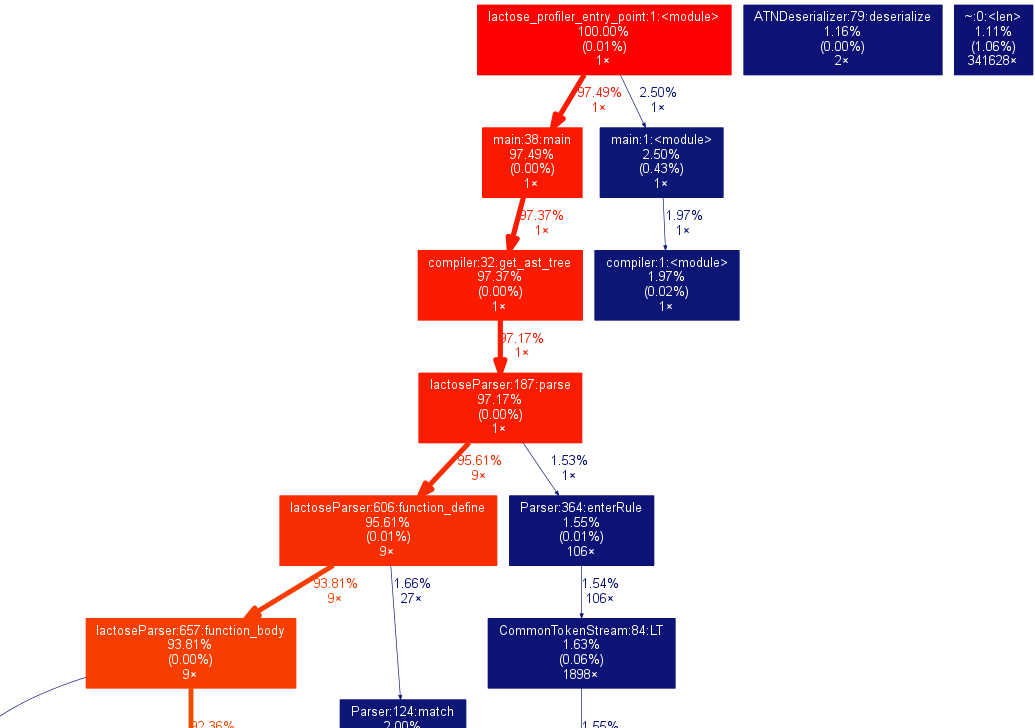
\includegraphics[scale=0.3]{lactose_stats.png}
            \caption{Результат работы профилировщика}
            \label{pic:stats}
        \end{figure}

        Вывод ANTLR для Python слоупок.
    
\clearpage

\section{Заключение}
    Что получилось. Привнесена няшность, но возможности далеко не такие как были.
\clearpage


\begin{thebibliography}{0}
\addcontentsline{toc}{section}{Список литературы}
    \bibitem{racket} Matthew Flatt, Robert Bruce Findler. The Racket Guide. Racket Documentation: URL: http://docs.racket-lang.org/guide/index.html.
    \bibitem{r5rs} R. Kelsey, W. Clinger, J. Rees. Revised$^5$ Report on the Algorithmic Language Scheme. Higher-Order and Symbolic Computation, Vol. 11, No. 1, August, 1998
    \bibitem{antlr} Terence Parr. The Definitive ANTLR 4 Reference. 2013.
    \bibitem{dragon} Ахо, Альфред В., Лам, Моника С., Сети, Рави, Ульман, Джеффри Д. Компиляторы: принципы, технологии и инструментарий, 2-е изд.: Пер. с англ.~--~М.: ООО <<И.Д.Вильямс>>, 2008~--~1184 с.
        
\end{thebibliography}

\end{document}
